% Options for packages loaded elsewhere
\PassOptionsToPackage{unicode}{hyperref}
\PassOptionsToPackage{hyphens}{url}
%
\documentclass[
  ignorenonframetext,
]{beamer}
\usepackage{pgfpages}
\setbeamertemplate{caption}[numbered]
\setbeamertemplate{caption label separator}{: }
\setbeamercolor{caption name}{fg=normal text.fg}
\beamertemplatenavigationsymbolsempty
% Prevent slide breaks in the middle of a paragraph
\widowpenalties 1 10000
\raggedbottom
\setbeamertemplate{part page}{
  \centering
  \begin{beamercolorbox}[sep=16pt,center]{part title}
    \usebeamerfont{part title}\insertpart\par
  \end{beamercolorbox}
}
\setbeamertemplate{section page}{
  \centering
  \begin{beamercolorbox}[sep=12pt,center]{part title}
    \usebeamerfont{section title}\insertsection\par
  \end{beamercolorbox}
}
\setbeamertemplate{subsection page}{
  \centering
  \begin{beamercolorbox}[sep=8pt,center]{part title}
    \usebeamerfont{subsection title}\insertsubsection\par
  \end{beamercolorbox}
}
\AtBeginPart{
  \frame{\partpage}
}
\AtBeginSection{
  \ifbibliography
  \else
    \frame{\sectionpage}
  \fi
}
\AtBeginSubsection{
  \frame{\subsectionpage}
}
\usepackage{amsmath,amssymb}
\usepackage{iftex}
\ifPDFTeX
  \usepackage[T1]{fontenc}
  \usepackage[utf8]{inputenc}
  \usepackage{textcomp} % provide euro and other symbols
\else % if luatex or xetex
  \usepackage{unicode-math} % this also loads fontspec
  \defaultfontfeatures{Scale=MatchLowercase}
  \defaultfontfeatures[\rmfamily]{Ligatures=TeX,Scale=1}
\fi
\usepackage{lmodern}
\usetheme[]{Madrid}
\ifPDFTeX\else
  % xetex/luatex font selection
\fi
% Use upquote if available, for straight quotes in verbatim environments
\IfFileExists{upquote.sty}{\usepackage{upquote}}{}
\IfFileExists{microtype.sty}{% use microtype if available
  \usepackage[]{microtype}
  \UseMicrotypeSet[protrusion]{basicmath} % disable protrusion for tt fonts
}{}
\makeatletter
\@ifundefined{KOMAClassName}{% if non-KOMA class
  \IfFileExists{parskip.sty}{%
    \usepackage{parskip}
  }{% else
    \setlength{\parindent}{0pt}
    \setlength{\parskip}{6pt plus 2pt minus 1pt}}
}{% if KOMA class
  \KOMAoptions{parskip=half}}
\makeatother
\usepackage{xcolor}
\newif\ifbibliography
\usepackage{color}
\usepackage{fancyvrb}
\newcommand{\VerbBar}{|}
\newcommand{\VERB}{\Verb[commandchars=\\\{\}]}
\DefineVerbatimEnvironment{Highlighting}{Verbatim}{commandchars=\\\{\}}
% Add ',fontsize=\small' for more characters per line
\usepackage{framed}
\definecolor{shadecolor}{RGB}{248,248,248}
\newenvironment{Shaded}{\begin{snugshade}}{\end{snugshade}}
\newcommand{\AlertTok}[1]{\textcolor[rgb]{0.94,0.16,0.16}{#1}}
\newcommand{\AnnotationTok}[1]{\textcolor[rgb]{0.56,0.35,0.01}{\textbf{\textit{#1}}}}
\newcommand{\AttributeTok}[1]{\textcolor[rgb]{0.13,0.29,0.53}{#1}}
\newcommand{\BaseNTok}[1]{\textcolor[rgb]{0.00,0.00,0.81}{#1}}
\newcommand{\BuiltInTok}[1]{#1}
\newcommand{\CharTok}[1]{\textcolor[rgb]{0.31,0.60,0.02}{#1}}
\newcommand{\CommentTok}[1]{\textcolor[rgb]{0.56,0.35,0.01}{\textit{#1}}}
\newcommand{\CommentVarTok}[1]{\textcolor[rgb]{0.56,0.35,0.01}{\textbf{\textit{#1}}}}
\newcommand{\ConstantTok}[1]{\textcolor[rgb]{0.56,0.35,0.01}{#1}}
\newcommand{\ControlFlowTok}[1]{\textcolor[rgb]{0.13,0.29,0.53}{\textbf{#1}}}
\newcommand{\DataTypeTok}[1]{\textcolor[rgb]{0.13,0.29,0.53}{#1}}
\newcommand{\DecValTok}[1]{\textcolor[rgb]{0.00,0.00,0.81}{#1}}
\newcommand{\DocumentationTok}[1]{\textcolor[rgb]{0.56,0.35,0.01}{\textbf{\textit{#1}}}}
\newcommand{\ErrorTok}[1]{\textcolor[rgb]{0.64,0.00,0.00}{\textbf{#1}}}
\newcommand{\ExtensionTok}[1]{#1}
\newcommand{\FloatTok}[1]{\textcolor[rgb]{0.00,0.00,0.81}{#1}}
\newcommand{\FunctionTok}[1]{\textcolor[rgb]{0.13,0.29,0.53}{\textbf{#1}}}
\newcommand{\ImportTok}[1]{#1}
\newcommand{\InformationTok}[1]{\textcolor[rgb]{0.56,0.35,0.01}{\textbf{\textit{#1}}}}
\newcommand{\KeywordTok}[1]{\textcolor[rgb]{0.13,0.29,0.53}{\textbf{#1}}}
\newcommand{\NormalTok}[1]{#1}
\newcommand{\OperatorTok}[1]{\textcolor[rgb]{0.81,0.36,0.00}{\textbf{#1}}}
\newcommand{\OtherTok}[1]{\textcolor[rgb]{0.56,0.35,0.01}{#1}}
\newcommand{\PreprocessorTok}[1]{\textcolor[rgb]{0.56,0.35,0.01}{\textit{#1}}}
\newcommand{\RegionMarkerTok}[1]{#1}
\newcommand{\SpecialCharTok}[1]{\textcolor[rgb]{0.81,0.36,0.00}{\textbf{#1}}}
\newcommand{\SpecialStringTok}[1]{\textcolor[rgb]{0.31,0.60,0.02}{#1}}
\newcommand{\StringTok}[1]{\textcolor[rgb]{0.31,0.60,0.02}{#1}}
\newcommand{\VariableTok}[1]{\textcolor[rgb]{0.00,0.00,0.00}{#1}}
\newcommand{\VerbatimStringTok}[1]{\textcolor[rgb]{0.31,0.60,0.02}{#1}}
\newcommand{\WarningTok}[1]{\textcolor[rgb]{0.56,0.35,0.01}{\textbf{\textit{#1}}}}
\usepackage{longtable,booktabs,array}
\usepackage{calc} % for calculating minipage widths
\usepackage{caption}
% Make caption package work with longtable
\makeatletter
\def\fnum@table{\tablename~\thetable}
\makeatother
\usepackage{graphicx}
\makeatletter
\def\maxwidth{\ifdim\Gin@nat@width>\linewidth\linewidth\else\Gin@nat@width\fi}
\def\maxheight{\ifdim\Gin@nat@height>\textheight\textheight\else\Gin@nat@height\fi}
\makeatother
% Scale images if necessary, so that they will not overflow the page
% margins by default, and it is still possible to overwrite the defaults
% using explicit options in \includegraphics[width, height, ...]{}
\setkeys{Gin}{width=\maxwidth,height=\maxheight,keepaspectratio}
% Set default figure placement to htbp
\makeatletter
\def\fps@figure{htbp}
\makeatother
\setlength{\emergencystretch}{3em} % prevent overfull lines
\providecommand{\tightlist}{%
  \setlength{\itemsep}{0pt}\setlength{\parskip}{0pt}}
\setcounter{secnumdepth}{-\maxdimen} % remove section numbering
\logo{
\includegraphics[height=1cm,width=3cm]{logo.png}}
\usetheme{Madrid}
\usefonttheme{serif}
\setbeamertemplate{navigation symbols}{}

\usepackage{amsmath}


\ifLuaTeX
  \usepackage{selnolig}  % disable illegal ligatures
\fi
\IfFileExists{bookmark.sty}{\usepackage{bookmark}}{\usepackage{hyperref}}
\IfFileExists{xurl.sty}{\usepackage{xurl}}{} % add URL line breaks if available
\urlstyle{same}
\hypersetup{
  pdftitle={Leksioni 2},
  pdfauthor={Endri Raco},
  hidelinks,
  pdfcreator={LaTeX via pandoc}}

\title{Leksioni 2}
\author{Endri Raco}
\date{23 April, 2024}

\begin{document}
\frame{\titlepage}

\begin{frame}[allowframebreaks]
  \tableofcontents[hideallsubsections]
\end{frame}
\hypertarget{kushtet-nuxeb-python}{%
\section{Kushtet në Python}\label{kushtet-nuxeb-python}}

\begin{frame}{Përmbledhje e Deklaratave të Kushtëzuara (Conditional
Statements)}
\protect\hypertarget{puxebrmbledhje-e-deklaratave-tuxeb-kushtuxebzuara-conditional-statements}{}
\begin{itemize}
\item
  Deklaratat kushtetuese në Python (if, elif, else) mundësojnë marrjen e
  vendimeve në kod.
\item
  Ato vlerësojnë kushte Booleane (True ose False) për të përcaktuar
  rrugët e ekzekutimit të kodit.
\end{itemize}
\end{frame}

\begin{frame}{Bazat e Deklaratave të Kushtëzuara}
\protect\hypertarget{bazat-e-deklaratave-tuxeb-kushtuxebzuara}{}
\begin{itemize}
\item
  e Deklaratave e Kushtëzuara mund të ndryshojnë sjelljen e kodit bazuar
  në kushte të caktuara.
\item
  Struktura bazë: NËSE një kusht plotësohet, ATËHERË një grup veprimesh
  ekzekutohet.
\end{itemize}
\end{frame}

\begin{frame}[fragile]{Deklaratë e Thjeshtë me Kusht}
\protect\hypertarget{deklaratuxeb-e-thjeshtuxeb-me-kusht}{}
Shembull i thjeshtë për temperaturën, për të parë nëse është e nxehtë
apo jo:

\begin{Shaded}
\begin{Highlighting}[]
\NormalTok{temperatura }\OperatorTok{=} \DecValTok{17}
\ControlFlowTok{if}\NormalTok{ temperatura }\OperatorTok{\textgreater{}} \DecValTok{25}\NormalTok{:}
    \BuiltInTok{print}\NormalTok{(}\StringTok{"është nxehtë!"}\NormalTok{)}
\ControlFlowTok{else}\NormalTok{:}
    \BuiltInTok{print}\NormalTok{(}\StringTok{"nuk është nxehtë!"}\NormalTok{)}
\end{Highlighting}
\end{Shaded}
\end{frame}

\begin{frame}{Deklaratë e Thjeshtë me Kusht}
\protect\hypertarget{deklaratuxeb-e-thjeshtuxeb-me-kusht-1}{}
\begin{itemize}
\item
  Fillimisht, përdorëm deklaratat \textbf{if} dhe \textbf{else} për të
  vendosur cilat pjesë të kodit të ekzekutohen.
\item
  Deklarata \textbf{if} kontrollon për të parë nëse vlera e variablës
  për temperaturën është më e madhe se 25.
\item
  Nëse ky kusht është i plotësuar, `është nxehtë' do të shkruhet në
  ekran.
\item
  Mqs 17 është më e vogël se 25, kodit nën \textbf{else} ekzekutohet.
\end{itemize}
\end{frame}

\begin{frame}{Deklaratë e Thjeshtë me Kusht}
\protect\hypertarget{deklaratuxeb-e-thjeshtuxeb-me-kusht-2}{}
\begin{itemize}
\item
  Kodi nën deklaratën \textbf{else} do të ekzekutohet kur testi i
  \textbf{if} është i pasaktë.
\item
  Le të përditësojmë temperaturën në një temperaturë ``e nxehtë'' dhe të
  përsërisim të njëjtën proces:
\end{itemize}
\end{frame}

\begin{frame}[fragile]{Deklaratë e Thjeshtë me Kusht}
\protect\hypertarget{deklaratuxeb-e-thjeshtuxeb-me-kusht-3}{}
\begin{Shaded}
\begin{Highlighting}[]
\NormalTok{temperatura }\OperatorTok{=} \DecValTok{30}
\ControlFlowTok{if}\NormalTok{ temperatura }\OperatorTok{\textgreater{}} \DecValTok{25}\NormalTok{:}
    \BuiltInTok{print}\NormalTok{(}\StringTok{"është nxehtë!"}\NormalTok{)}
\ControlFlowTok{else}\NormalTok{:}
    \BuiltInTok{print}\NormalTok{(}\StringTok{"nuk është nxehtë!"}\NormalTok{)}
\end{Highlighting}
\end{Shaded}
\end{frame}

\begin{frame}{Deklaratat If pa Else}
\protect\hypertarget{deklaratat-if-pa-else}{}
\begin{itemize}
\item
  \textbf{Else} nuk është gjithmonë i nevojshëm në deklaratat e
  Kushtëzuara.
\item
  Nëse kushti është \textbf{False} dhe nuk ka \textbf{Else}, Python nuk
  bën asgjë.
\end{itemize}
\end{frame}

\begin{frame}[fragile]{Deklaratat If pa Else}
\protect\hypertarget{deklaratat-if-pa-else-1}{}
\begin{Shaded}
\begin{Highlighting}[]
\NormalTok{temperature }\OperatorTok{=} \DecValTok{17}

\ControlFlowTok{if}\NormalTok{ temperature }\OperatorTok{\textgreater{}} \DecValTok{25}\NormalTok{:}
  \BuiltInTok{print}\NormalTok{(temperature, }\StringTok{"është më shume se 25"}\NormalTok{)  }
\end{Highlighting}
\end{Shaded}
\end{frame}

\begin{frame}{Deklaratat If pa Else}
\protect\hypertarget{deklaratat-if-pa-else-2}{}
\begin{itemize}
\item
  Deklaratat e kushtëzuara gjithmonë kontrollojnë nëse shprehja e
  kushtëzuar është e vërtetë ose e gabuar.
\item
  Nëse është e vërtetë, blloku i kodit nën deklaratën e kushtëzuar
  ekzekutohet.
\item
  Asgjë nuk printohet në ekran nëse temperatura është më e vogël se 25.
\end{itemize}
\end{frame}

\begin{frame}{Deklaratat If pa Else}
\protect\hypertarget{deklaratat-if-pa-else-3}{}
Imagjinoni që jeni duke u përgatitur për të dalë nga shtëpia dhe
dëshironi të vendosni çfarë të vishni.

\begin{itemize}
\item
  Mund të shikoni jashtë për të kontrolluar kushtet e motit.
\item
  Nëse po bie shi, do të vishni një xhaketë shiu.
\end{itemize}
\end{frame}

\begin{frame}[fragile]{Shembull}
\protect\hypertarget{shembull}{}
Python-i përdor operatorin \textbf{==} për të provuar nëse një vlerë
është e barabartë me një tjetër.

\begin{Shaded}
\begin{Highlighting}[]
\NormalTok{moti }\OperatorTok{=} \StringTok{"shi"}

\ControlFlowTok{if}\NormalTok{ moti }\OperatorTok{==} \StringTok{"shi"}\NormalTok{:}
  \BuiltInTok{print}\NormalTok{(}\StringTok{"Vish një xhaketë shiu!"}\NormalTok{)}
\ControlFlowTok{else}\NormalTok{:}
  \BuiltInTok{print}\NormalTok{(}\StringTok{"Nuk ka nevojë për xhaketën e shiut."}\NormalTok{)}
\end{Highlighting}
\end{Shaded}
\end{frame}

\begin{frame}{Deklaratat e kushtëzuara}
\protect\hypertarget{deklaratat-e-kushtuxebzuara}{}
\begin{itemize}
\item
  Njësoj si me ciklin \textbf{for}, Python-i përdor \textbf{(:)} dhe
  hapësirën e bardhë (indentimet; shpesh katër hapësira) për të
  strukturuar deklaratat e kushtëzuara.
\item
  Nëse kushti është i vërtetë, blloku i kodit i shkruar me indentim pas
  colon (:) ekzekutohet.
\end{itemize}
\end{frame}

\begin{frame}{Deklaratat e kushtëzuara}
\protect\hypertarget{deklaratat-e-kushtuxebzuara-1}{}
\begin{itemize}
\tightlist
\item
  Blloku i kodit mund të përmbajë disa rreshta kodi, por të gjithë duhet
  të jenë të indentuar identikisht.
\end{itemize}

Do të merrni një \textbf{IndentationError}, një \textbf{SyntaxError},
ose sjellje të pa dëshiruara nëse nuk e keni indentuar kodin tuaj në
mënyrë të saktë.
\end{frame}

\begin{frame}{Deklaratat e kushtëzuara}
\protect\hypertarget{deklaratat-e-kushtuxebzuara-2}{}
\begin{itemize}
\item
  Duhet pasur kujdes që edhe teksti që krahasohet (shkronjat e mëdha ose
  të vogla) janë të rëndësishme.
\item
  Për shembull, në shembullin më sipër, nëse ne definonim \textbf{motin
  = `Shi'}, krahasimi \textbf{moti == `shi'} do të ishte i gabuar.
\item
  \begin{itemize}
  \tightlist
  \item
    Një zgjidhje e mundshme për këtë problem është përdorimi i metodës
    \textbf{.lower()} për stringje, e cila do të konvertojë tekstin në
    të cilin aplikohet në shkronja të vogla.
  \end{itemize}
\end{itemize}
\end{frame}

\begin{frame}[fragile]{Deklaratat e kushtëzuara}
\protect\hypertarget{deklaratat-e-kushtuxebzuara-3}{}
\begin{Shaded}
\begin{Highlighting}[]
\NormalTok{moti }\OperatorTok{=} \StringTok{"Shi"}

\ControlFlowTok{if}\NormalTok{  moti.lower() }\OperatorTok{==} \StringTok{\textquotesingle{}shi\textquotesingle{}}\NormalTok{:}
  \BuiltInTok{print}\NormalTok{(}\StringTok{"Vish një xhaketë shiu!"}\NormalTok{)}
\ControlFlowTok{else}\NormalTok{:}
  \BuiltInTok{print}\NormalTok{(}\StringTok{"Nuk ka nevojë për xhaketën e shiut."}\NormalTok{)}
\end{Highlighting}
\end{Shaded}
\end{frame}

\begin{frame}{Operatorët krahasues}
\protect\hypertarget{operatoruxebt-krahasues}{}
\begin{itemize}
\tightlist
\item
  Operatorët krahasues si \textbf{\textgreater{}} dhe \textbf{==}
  krahasojnë vlerat në të dy anët e operatorit.
\end{itemize}

\begin{longtable}[]{@{}ll@{}}
\toprule\noalign{}
Operatori & Përshkrimi \\
\midrule\noalign{}
\endhead
\textless{} & Më pak se \\
\textless= & Më pak se ose e barabartë me \\
== & E barabartë me \\
\textgreater= & Më e madhe se ose e barabartë me \\
\textgreater{} & Më e madhe se \\
!= & Jo e barabartë me \\
\bottomrule\noalign{}
\end{longtable}
\end{frame}

\begin{frame}{Vlerat Booleane}
\protect\hypertarget{vlerat-booleane}{}
\begin{itemize}
\item
  Operacionet krahasuese japin vlera booleane \textbf{(True ose False)}.
\item
  Në Python, fjalët \textbf{True} dhe \textbf{False} janë të rezervuara
  për këto vlera Booleane dhe nuk mund të përdoren për asgjë tjetër.
\end{itemize}
\end{frame}

\begin{frame}[fragile]{Vlerat Booleane}
\protect\hypertarget{vlerat-booleane-1}{}
Le të kontrollojmë vlerën aktuale të kushteve që përdorëm në shembujt e
mëparshëm:

\begin{Shaded}
\begin{Highlighting}[]
\NormalTok{temperature }\OperatorTok{\textgreater{}} \DecValTok{25}

\NormalTok{moti }\OperatorTok{==} \StringTok{"shi"}
\end{Highlighting}
\end{Shaded}
\end{frame}

\begin{frame}[fragile]{If, elif dhe else:}
\protect\hypertarget{if-elif-dhe-else}{}
\begin{itemize}
\item
  Mund të lidhim disa kushte së bashku duke përdorur deklaratën ``else
  if'' - elif.
\item
  Python-i kontrollon deklaratat \textbf{elif} dhe \textbf{else} vetëm
  nëse kushtet e mëparshme ishin të pavërteta.
\item
  Mund të kemi shumë deklarata \textbf{elif} për të kontrolluar kushte
  shtesë.
\end{itemize}

\begin{Shaded}
\begin{Highlighting}[]
\NormalTok{temperature }\OperatorTok{=} \OperatorTok{{-}}\DecValTok{3}
\ControlFlowTok{if}\NormalTok{ temperature }\OperatorTok{\textgreater{}} \DecValTok{0}\NormalTok{:}
    \BuiltInTok{print}\NormalTok{(temperature, }\StringTok{"gradë Celsius janë mbi temperatura e ftohjes"}\NormalTok{)}
\ControlFlowTok{elif}\NormalTok{ temperature }\OperatorTok{==} \DecValTok{0}\NormalTok{:}
    \BuiltInTok{print}\NormalTok{(temperature, }\StringTok{"gradë Celsius janë në pikën e ftohjes"}\NormalTok{)}
\ControlFlowTok{else}\NormalTok{:}
    \BuiltInTok{print}\NormalTok{(temperature, }\StringTok{"gradë Celsius janë poshtë temperatures së ftohjes"}\NormalTok{)}
\end{Highlighting}
\end{Shaded}

\begin{verbatim}
-3 gradë Celsius janë poshtë temperatures së ftohjes
\end{verbatim}
\end{frame}

\begin{frame}{Kombinimi i kushteve}
\protect\hypertarget{kombinimi-i-kushteve}{}
\begin{itemize}
\tightlist
\item
  Ne gjithashtu mund të përdorim \textbf{and} dhe \textbf{or} për të
  kombinuar kushte të shumëfishta në vlera boolean
\end{itemize}

\begin{longtable}[]{@{}
  >{\raggedright\arraybackslash}p{(\columnwidth - 4\tabcolsep) * \real{0.2927}}
  >{\centering\arraybackslash}p{(\columnwidth - 4\tabcolsep) * \real{0.2683}}
  >{\raggedright\arraybackslash}p{(\columnwidth - 4\tabcolsep) * \real{0.4390}}@{}}
\caption{\emph{\textbf{Tabela}. Logjika për fjalëkalimet and dhe or në
Python.}}\tabularnewline
\toprule\noalign{}
\begin{minipage}[b]{\linewidth}\raggedright
Fjalëkalim
\end{minipage} & \begin{minipage}[b]{\linewidth}\centering
Shembull
\end{minipage} & \begin{minipage}[b]{\linewidth}\raggedright
Përshkrim
\end{minipage} \\
\midrule\noalign{}
\endfirsthead
\toprule\noalign{}
\begin{minipage}[b]{\linewidth}\raggedright
Fjalëkalim
\end{minipage} & \begin{minipage}[b]{\linewidth}\centering
Shembull
\end{minipage} & \begin{minipage}[b]{\linewidth}\raggedright
Përshkrim
\end{minipage} \\
\midrule\noalign{}
\endhead
and & a and b & E vërtetë nëse të dy a dhe b janë të vërteta \\
or & a or b & E vërtetë nëse a ose b është e vërtetë \\
\bottomrule\noalign{}
\end{longtable}
\end{frame}

\begin{frame}[fragile]{Kombinimi i kushteve}
\protect\hypertarget{kombinimi-i-kushteve-1}{}
\begin{Shaded}
\begin{Highlighting}[]
\ControlFlowTok{if}\NormalTok{ (}\DecValTok{1} \OperatorTok{\textgreater{}} \DecValTok{0}\NormalTok{) }\KeywordTok{and}\NormalTok{ (}\OperatorTok{{-}}\DecValTok{1} \OperatorTok{\textgreater{}} \DecValTok{0}\NormalTok{):}
    \BuiltInTok{print}\NormalTok{(}\StringTok{"Të dy pjesët janë të vërteta"}\NormalTok{)}
\ControlFlowTok{else}\NormalTok{:}
    \BuiltInTok{print}\NormalTok{(}\StringTok{"Të paktën një pjesë nuk është e vërtetë"}\NormalTok{)}
\end{Highlighting}
\end{Shaded}

\begin{verbatim}
Të paktën një pjesë nuk është e vërtetë
\end{verbatim}
\end{frame}

\begin{frame}[fragile]{Kombinimi i for-loops dhe deklaratave kushtore}
\protect\hypertarget{kombinimi-i-for-loops-dhe-deklaratave-kushtore}{}
\begin{itemize}
\item
  Gjithashtu mund të kombinojmë \textbf{for-loops} dhe deklarata
  kushtore.
\item
  Le të iterojmë nëpër një listë temperature dhe të kontrollojmë nëse
  temperatura është e nxehtë apo jo:
\end{itemize}

\begin{Shaded}
\begin{Highlighting}[]
\NormalTok{temperatura }\OperatorTok{=}\NormalTok{ [}\DecValTok{0}\NormalTok{, }\DecValTok{12}\NormalTok{, }\DecValTok{17}\NormalTok{, }\DecValTok{28}\NormalTok{, }\DecValTok{30}\NormalTok{]}

\CommentTok{\# Për çdo temperaturë, nëse temperatura është më e madhe se 25, printo "..është e nxehtë"}
\ControlFlowTok{for}\NormalTok{ temperatura }\KeywordTok{in}\NormalTok{ temperatura:}
    \ControlFlowTok{if}\NormalTok{ temperatura }\OperatorTok{\textgreater{}} \DecValTok{25}\NormalTok{:}
        \BuiltInTok{print}\NormalTok{(temperatura, }\StringTok{"është e nxehtë"}\NormalTok{)}
    \ControlFlowTok{else}\NormalTok{:}
        \BuiltInTok{print}\NormalTok{(temperatura, }\StringTok{"nuk është e nxehtë"}\NormalTok{)}
\end{Highlighting}
\end{Shaded}

\begin{verbatim}
0 nuk është e nxehtë
12 nuk është e nxehtë
17 nuk është e nxehtë
28 është e nxehtë
30 është e nxehtë
\end{verbatim}
\end{frame}

\hypertarget{funksionet}{%
\section{Funksionet}\label{funksionet}}

\begin{frame}{Funksionet}
\protect\hypertarget{funksionet-1}{}
\begin{itemize}
\tightlist
\item
  Do prezantojmë funksionet si një mënyrë për të krijuar blloqe të kodit
  për një detyrë të caktuar që janë të lehta për tu përdorur dhe
  ripërdorur në programet tuaja.
\end{itemize}
\end{frame}

\begin{frame}{Çfarë është një funksion?}
\protect\hypertarget{uxe7faruxeb-uxebshtuxeb-njuxeb-funksion}{}
\begin{itemize}
\item
  Një funksion është një bllok kodi i organizuar, i ripërdorshëm që mund
  të bëjë programet tuaja më efektive, më të lehta për t'u lexuar dhe të
  thjeshta për t'u menaxhuar.
\item
  Mund ta mendojmë funksionin si program i vogë i pavarur që mund të
  kryejë një detyrë specifike dhe që mund të përdoret përsëri në kodin
  tuaj.
\end{itemize}
\end{frame}

\begin{frame}{Çfarë është një funksion?}
\protect\hypertarget{uxe7faruxeb-uxebshtuxeb-njuxeb-funksion-1}{}
\begin{itemize}
\item
  Një nga principet themelore në programimin e mirë është ``mos e
  përsërisni veten''.
\item
  Me fjalë të tjera, duhet të shmangni linja kodi të përsëritura në
  skriptet tuaja.
\end{itemize}
\end{frame}

\begin{frame}{Çfarë është një funksion?}
\protect\hypertarget{uxe7faruxeb-uxebshtuxeb-njuxeb-funksion-2}{}
\begin{itemize}
\tightlist
\item
  Funksionet janë një mënyrë e mirë për të shmangur situata të tilla dhe
  kursejnë kohë dhe përpjekje, pasi nuk ju nevojitet të tregoni
  kompjuterit përsëri çfarë të bëjë çdo herë që bën një detyrë të
  zakonshme, si konvertimi i temperaturave nga Fahrenheit në Celsius.
\end{itemize}
\end{frame}

\begin{frame}{Anatomia e një funksioni}
\protect\hypertarget{anatomia-e-njuxeb-funksioni}{}
\begin{itemize}
\item
  Le të shohim përsëri detyrën e konvertimit të temperaturave nga
  Celsius në Fahrenheit.
\item
  Një operacion i tillë është një detyrë e zakonshme kur punojmë me të
  dhënat e temperaturës.
\item
  Prandaj mund të nevojitet të përsërisim këto llogaritje shpesh kur
  analizojmë ose krahasojmë të dhëna të motit ose klimës midis
  Shqipërisë dhe Greqisë, për shembull.
\end{itemize}
\end{frame}

\begin{frame}[fragile]{Krijimi i funksionit të parë}
\protect\hypertarget{krijimi-i-funksionit-tuxeb-paruxeb}{}
\begin{itemize}
\tightlist
\item
  Le të përcaktojmë funksionin tonë të parë të quajtur
  \textbf{cel\_ne\_farh}.
\end{itemize}

\begin{Shaded}
\begin{Highlighting}[]
\KeywordTok{def}\NormalTok{ cel\_ne\_farh(temp):}
    \ControlFlowTok{return} \DecValTok{9} \OperatorTok{/} \DecValTok{5} \OperatorTok{*}\NormalTok{ temp }\OperatorTok{+} \DecValTok{32}
\end{Highlighting}
\end{Shaded}
\end{frame}

\begin{frame}{Thirrja e një funksioni}
\protect\hypertarget{thirrja-e-njuxeb-funksioni}{}
\begin{itemize}
\item
  Tani le të provojmë të përdorim funksionin tonë.
\item
  Thirrja e funksionit të paracaktuar nuk është ndryshe nga thirrja e
  ndonjë funksioni tjetër siç është \textbf{print()}.
\item
  Duhet ta thërresim me emrin e tij dhe të siguroni vlerën/vlerat tuaja
  si parametrat e kërkuara brenda thonjëzave.
\end{itemize}
\end{frame}

\begin{frame}[fragile]{Thirrja e një funksioni}
\protect\hypertarget{thirrja-e-njuxeb-funksioni-1}{}
\begin{Shaded}
\begin{Highlighting}[]
\NormalTok{pike\_ngrirje }\OperatorTok{=}\NormalTok{ cel\_ne\_farh(}\DecValTok{0}\NormalTok{)}
\BuiltInTok{print}\NormalTok{(}\StringTok{"Pika e ngrirjes së ujit në Fahrenheit është:"}\NormalTok{, pike\_ngrirje)}
\end{Highlighting}
\end{Shaded}
\end{frame}

\begin{frame}[fragile]{Krijimi i një funksioni tjetër}
\protect\hypertarget{krijimi-i-njuxeb-funksioni-tjetuxebr}{}
\begin{itemize}
\tightlist
\item
  Tani që e dimë si të krijojmë një funksion për të konvertuar Celsius
  në Fahrenheit, le të krijojmë një funksion tjetër të quajtur
  \textbf{kelv\_ne\_cel}.
\end{itemize}

\begin{Shaded}
\begin{Highlighting}[]
\KeywordTok{def}\NormalTok{ kelv\_ne\_cel(temp\_kelv):}
    \ControlFlowTok{return}\NormalTok{ temp\_kelv }\OperatorTok{{-}} \FloatTok{273.15}
\end{Highlighting}
\end{Shaded}
\end{frame}

\begin{frame}[fragile]{Krijimi i një funksioni tjetër}
\protect\hypertarget{krijimi-i-njuxeb-funksioni-tjetuxebr-1}{}
\begin{itemize}
\tightlist
\item
  E përdorim në të njëjtën mënyrë si më herët duke përcaktuar një
  variabël të ri \textbf{zero\_absolute} që është temperatura Celsius e
  0 Kelvins.
\end{itemize}

\begin{Shaded}
\begin{Highlighting}[]
\NormalTok{zero\_absolute }\OperatorTok{=}\NormalTok{ kelv\_ne\_cel(temp\_kelv}\OperatorTok{=}\DecValTok{0}\NormalTok{)}
\BuiltInTok{print}\NormalTok{(}\StringTok{"Zero absolut në Celsius është:"}\NormalTok{, zero\_absolute)}
\end{Highlighting}
\end{Shaded}
\end{frame}

\begin{frame}{Funksionet brenda funksionit}
\protect\hypertarget{funksionet-brenda-funksionit}{}
\begin{itemize}
\item
  Si do vepronim për konvertimin e Kelvins në Fahrenheit?
\item
  Ne mund të shkruajmë një formulë për këtë, por nuk kemi nevojë.
\end{itemize}
\end{frame}

\begin{frame}{Funksionet brenda funksionit}
\protect\hypertarget{funksionet-brenda-funksionit-1}{}
\begin{itemize}
\item
  Në vend të kësaj, mund të bëjmë konvertimin duke përdorur dy
  funksionet që kemi krijuar tashmë dhe duke i thirrur ato nga funksioni
  që po krijojmë tani.
\item
  Le të krijojmë një funksion të ri \textbf{kelv\_ne\_fahr} që merr
  temperaturën në Kelvins si parametër \textbf{temp\_kelv} dhe përdor
  funksionet tona \textbf{kelv\_ne\_cel} dhe \textbf{cel\_ne\_farh}
  brenda funksionit të ri për të konvertuar temperaturat nga Kelvins në
  Fahrenheit.
\end{itemize}
\end{frame}

\begin{frame}[fragile]{Funksionet brenda funksionit}
\protect\hypertarget{funksionet-brenda-funksionit-2}{}
\begin{Shaded}
\begin{Highlighting}[]
\KeywordTok{def}\NormalTok{ kelv\_ne\_fahr(temp\_kelv):}
\NormalTok{    temp\_cels }\OperatorTok{=}\NormalTok{ kelv\_ne\_cel(temp\_kelv)}
\NormalTok{    temp\_fahr }\OperatorTok{=}\NormalTok{ cel\_ne\_farh(temp\_cels)}
    \ControlFlowTok{return}\NormalTok{ temp\_fahr}
\end{Highlighting}
\end{Shaded}
\end{frame}

\begin{frame}{Funksionet brenda funksionit}
\protect\hypertarget{funksionet-brenda-funksionit-3}{}
\begin{itemize}
\item
  Tani le të përdorim funksionin për të llogaritur temperaturën zero
  absolute në gradë Fahrenheit.
\item
  Pastaj mund ta printojmë atë vlerë në ekran përsëri.
\end{itemize}
\end{frame}

\begin{frame}[fragile]{Funksionet brenda funksionit}
\protect\hypertarget{funksionet-brenda-funksionit-4}{}
\begin{Shaded}
\begin{Highlighting}[]
\NormalTok{zero\_abs\_fahr }\OperatorTok{=}\NormalTok{ kelv\_ne\_fahr(temp\_kelv}\OperatorTok{=}\DecValTok{0}\NormalTok{)}
\BuiltInTok{print}\NormalTok{(}\StringTok{"Zeroja absolute në Fahrenheit është:"}\NormalTok{, zero\_abs\_fahr)}
\end{Highlighting}
\end{Shaded}
\end{frame}

\begin{frame}{Funksionet dhe emrat e variablave}
\protect\hypertarget{funksionet-dhe-emrat-e-variablave}{}
\begin{itemize}
\tightlist
\item
  Një pikë e zakonshme e konfuzionit për programuesit e rinj është
  kuptimi se si emrat e variablave në funksione lidhen me ato që janë
  përcaktuar në vende të tjera të shënimet tuaja.
\end{itemize}

\emph{Kur përcaktohet një funksion, emrat e variablave të dhënë në
definicionin e funksionit ekzistojnë dhe do të përdoren vetëm kur
funksioni thirret}

\begin{itemize}
\tightlist
\item
  Le ta kuptojmë këtë me një shembull.
\end{itemize}
\end{frame}

\begin{frame}[fragile]{Definimi i një funksioni të modifikuar}
\protect\hypertarget{definimi-i-njuxeb-funksioni-tuxeb-modifikuar}{}
\begin{itemize}
\tightlist
\item
  Le të përcaktojmë një version të modifikuar të funksionit tonë
  \textbf{kelv\_ne\_cel}, ku vlera e parametrit vazhdon të quhet
  \textbf{temp\_kelv}, por tani së pari do ruajmë temperaturën e
  konvertuar si \textbf{temp\_cels} dhe do kthejmë atë vlerë.
\end{itemize}

\begin{Shaded}
\begin{Highlighting}[]
\KeywordTok{def}\NormalTok{ kelv\_ne\_cel(temp\_kelv):}
\NormalTok{    temp\_cels }\OperatorTok{=}\NormalTok{ temp\_kelv }\OperatorTok{{-}} \FloatTok{273.15}
    \ControlFlowTok{return}\NormalTok{ temp\_cels}
\end{Highlighting}
\end{Shaded}
\end{frame}

\begin{frame}{Definimi i një funksioni të modifikuar}
\protect\hypertarget{definimi-i-njuxeb-funksioni-tuxeb-modifikuar-1}{}
\begin{itemize}
\item
  Pra, kemi përcaktuar funksionin tonë për të pranuar temp\_kelv si
  parametër të vetëm
\item
  Kemi llogaritur \textbf{temp\_cels}, dhe kthyer atë vlerë.
\end{itemize}
\end{frame}

\begin{frame}{Definimi i një funksioni të modifikuar}
\protect\hypertarget{definimi-i-njuxeb-funksioni-tuxeb-modifikuar-2}{}
\textbf{Por, variablat e përcaktuara në funksion ekzistojnë vetëm në
hapësirën e tij.}
\end{frame}

\begin{frame}[fragile]{Konfirmimi}
\protect\hypertarget{konfirmimi}{}
\begin{itemize}
\tightlist
\item
  Këtu, në hapësirën globale (global namespace), ne marrim një
  \textbf{NameError} kur përpiqemi të qasemi në variablat
  \textbf{temp\_kelv} ose \textbf{temp\_cels} sepse ato janë përcaktuar
  vetëm brenda funksionit \textbf{kelv\_ne\_cel}.
\end{itemize}

\begin{Shaded}
\begin{Highlighting}[]
\NormalTok{temp\_kelvins}
\NormalTok{temp\_celsius}
\CommentTok{\# Output: NameError: name \textquotesingle{}temp\_celsius\textquotesingle{} is not defined}
\end{Highlighting}
\end{Shaded}
\end{frame}

\begin{frame}{Definimi i një funksioni të modifikuar}
\protect\hypertarget{definimi-i-njuxeb-funksioni-tuxeb-modifikuar-3}{}
\begin{itemize}
\tightlist
\item
  Në këtë rast, edhe pse funksioni është përcaktuar, variablat brenda
  tij nuk janë në dispozicion jashtë tij.
\end{itemize}
\end{frame}

\begin{frame}[fragile]{Përdorimi i funksionit}
\protect\hypertarget{puxebrdorimi-i-funksionit}{}
\begin{itemize}
\tightlist
\item
  Tani le të përdorim funksionin për të parë nëse vlerat e këtyre
  variablave do të përcaktohen pasi të ketë ndodhur thirrja e
  funksionit.
\end{itemize}

\begin{Shaded}
\begin{Highlighting}[]
\NormalTok{kelv\_ne\_cel(temp\_kelv}\OperatorTok{=}\FloatTok{293.15}\NormalTok{)}
\CommentTok{\# Output: 20.0}
\NormalTok{temp\_kelv}
\CommentTok{\# Output: NameError: name \textquotesingle{}temp\_kelvins\textquotesingle{} is not defined}
\end{Highlighting}
\end{Shaded}
\end{frame}

\begin{frame}{Përdorimi i funksionit}
\protect\hypertarget{puxebrdorimi-i-funksionit-1}{}
\begin{itemize}
\tightlist
\item
  Siç mund të shihni, \textbf{temp\_kelv} ende nuk është i përcaktuar në
  hapësirën globale, ku vlera si \textbf{pike\_ngrirje} janë të
  përcaktuara.
\end{itemize}
\end{frame}

\begin{frame}{Pse punon Python-i kështu?}
\protect\hypertarget{pse-punon-python-i-kuxebshtu}{}
\begin{itemize}
\tightlist
\item
  Në Python, e mira e një hapësire të veçantë për funksionet është që
  mund të përcaktojmë një variabël në hapësirën globale, siç është
  \textbf{temp\_kelv}, dhe të mos kemi pse shqetësohemi për emrin e
  këtij variabli brenda një funksioni, ose përdorimin e një funksioni që
  e ndryshon vlerën e variablit.
\end{itemize}
\end{frame}

\begin{frame}{Pse punon Python-i kështu?}
\protect\hypertarget{pse-punon-python-i-kuxebshtu-1}{}
\begin{itemize}
\tightlist
\item
  Brenda funksionit, vlera që kalohet do të njihet si
  \textbf{temp\_kelv}, por ndryshimi i kësaj vlere nuk do të ndryshojë
  një variabël me të njëjtën emër në hapësirën globale.
\end{itemize}
\end{frame}

\begin{frame}[fragile]{Shembull}
\protect\hypertarget{shembull-1}{}
Le të shohim një shembull tjetër duke përdorur një funksion të
modifikuar \textbf{kelv\_ne\_cel2()}.

\begin{Shaded}
\begin{Highlighting}[]
\KeywordTok{def}\NormalTok{ kelv\_ne\_cel2(temperature):}
\NormalTok{    temperature }\OperatorTok{=}\NormalTok{ temperature }\OperatorTok{{-}} \FloatTok{273.15}
    \ControlFlowTok{return}\NormalTok{ temperature}
\end{Highlighting}
\end{Shaded}
\end{frame}

\begin{frame}[fragile]{Përdorimi i funksionit të modifikuar}
\protect\hypertarget{puxebrdorimi-i-funksionit-tuxeb-modifikuar}{}
\begin{itemize}
\tightlist
\item
  Tani le të përcaktojmë një variabël temperature në hapësirën globale
  dhe të përdorim funksionin tonë për ta ndryshuar atë.
\end{itemize}

\begin{Shaded}
\begin{Highlighting}[]
\NormalTok{temperature }\OperatorTok{=} \FloatTok{303.15}
\NormalTok{kelv\_ne\_cel2(temperature}\OperatorTok{=}\NormalTok{temperature)}
\CommentTok{\# Output: 30.0}

\NormalTok{temperature}
\CommentTok{\# Output: 303.15}
\end{Highlighting}
\end{Shaded}
\end{frame}

\begin{frame}{Përdorimi i funksionit të modifikuar}
\protect\hypertarget{puxebrdorimi-i-funksionit-tuxeb-modifikuar-1}{}
\begin{itemize}
\item
  Siç mund të shihni, vlera e variablit \textbf{temperature} në
  hapësirën globale ishte \textbf{303.15} dhe mbetet \textbf{303.15} pas
  përdorimit të funksionit \textbf{kelv\_ne\_cel2}.
\item
  Edhe pse ka një variabël brenda atij funksioni me të njëjtin emër si
  vlera në hapësirën globale, përdorimi i funksionit cakton vlerën e
  temperature brenda funksionit dhe manipulon atë vlerë vetëm brenda
  funksionit.
\end{itemize}
\end{frame}

\begin{frame}[fragile]{Mundësia për të qasur vlerat e variablave globale
në funksione}
\protect\hypertarget{munduxebsia-puxebr-tuxeb-qasur-vlerat-e-variablave-globale-nuxeb-funksione}{}
\begin{itemize}
\item
  Është e rëndësishme të kuptojmë se është e mundur të thërresim vlerat
  e variablave që janë të përcaktuara në hapësirën globale brenda
  funksioneve, edhe nëse vlera nuk është kaluar si argument në funksion.
\item
  Kjo ndodh sepse Python-i do të kërkojë për variablat e përcaktuara në
  hapësirën globale brenda funksioneve, dhe nëse gjen një variabël me
  emrin e dhënë, atëherë do ta përdorë atë në funksion.
\end{itemize}

\begin{block}{Shembuj}
\protect\hypertarget{shembuj}{}
\begin{Shaded}
\begin{Highlighting}[]
\CommentTok{\# Definimi i një variabli global}
\NormalTok{temperature }\OperatorTok{\textless{}{-}} \FloatTok{303.15}

\CommentTok{\# Definimi i një funksioni që përdor variabël global}
\NormalTok{kelv\_ne\_cel3 }\OperatorTok{\textless{}{-}}\NormalTok{ function(temp) \{}
\NormalTok{    temp }\OperatorTok{\textless{}{-}}\NormalTok{ temperature }\OperatorTok{{-}} \FloatTok{273.15}
    \ControlFlowTok{return}\NormalTok{(temp)}
\NormalTok{\}}

\CommentTok{\# Thirrja e funksionit dhe përdorimi i variablit  global}
\NormalTok{kelv\_ne\_cel3(}\FloatTok{273.15}\NormalTok{)  }\CommentTok{\# Output: 30.0}
\end{Highlighting}
\end{Shaded}
\end{block}
\end{frame}

\begin{frame}{Dokumentimi i funksioneve me docstrings}
\protect\hypertarget{dokumentimi-i-funksioneve-me-docstrings}{}
\begin{itemize}
\item
  Dokumentimi i funksioneve është i rëndësishëm për të kuptuar se çfarë
  bën një funksion, si dhe se si duhet të përdoret.
\item
  Një mënyrë e zakonshme për të dokumentuar funksionet në Python është
  përdorimi i \textbf{docstrings}.
\end{itemize}
\end{frame}

\begin{frame}[fragile]{Shembuj}
\protect\hypertarget{shembuj-1}{}
\begin{Shaded}
\begin{Highlighting}[]
\KeywordTok{def}\NormalTok{ kelv\_ne\_cel(temp\_kelv):}
    \CommentTok{"""}
\CommentTok{    Konverton temp nga Kelvin ne grade Celcius.}

\CommentTok{    Parametra}
\CommentTok{    {-}{-}{-}{-}{-}{-}{-}{-}{-}{-}}
\CommentTok{    temp\_kelv: \textless{}numerical\textgreater{}}
\CommentTok{        Temperatura ne Kelvin}

\CommentTok{    Kthen}
\CommentTok{    {-}{-}{-}{-}{-}{-}{-}}
\CommentTok{    \textless{}float\textgreater{}}
\CommentTok{        Temperatura e konvertuar}
\CommentTok{    """}
    \ControlFlowTok{return}\NormalTok{ temp\_kelv }\OperatorTok{{-}} \FloatTok{273.15}
\end{Highlighting}
\end{Shaded}
\end{frame}

\hypertarget{shkrimi-i-skripteve}{%
\section{Shkrimi i skripteve}\label{shkrimi-i-skripteve}}

\begin{frame}{Shkrimi i skripteve}
\protect\hypertarget{shkrimi-i-skripteve-1}{}
\begin{itemize}
\item
  Deri më tani kemi mbajtur kodin tonë Python dhe komentet Markdown në
  një dokument të vetëm të Jupyter notebook.
\item
  Kjo është ok, por ka raste kur kodi ynë Python është i gjatë ose kur
  kemi një set funksionesh të përdorura në shumë Jupyter notebooks
\end{itemize}
\end{frame}

\begin{frame}[fragile]{Shkrimi i skripteve}
\protect\hypertarget{shkrimi-i-skripteve-2}{}
\begin{itemize}
\item
  Në këto raste, mund të duam të kemi kodin Python në një dokument të
  veçantë
\item
  Alternativa për të shtypur të gjitha komandat që dëshironi të
  ekzekutoni është t'i listoni ato në një skedar Python
  \emph{\{term\}\texttt{skript}}.
\item
  Skedarët skript Python tradicionalisht përdorin zgjatjen e skedarit
  \texttt{.py} në emrat e tyre.
\end{itemize}
\end{frame}

\begin{frame}{Shkrimi i skripteve}
\protect\hypertarget{shkrimi-i-skripteve-3}{}
Së pari, duhet të krijoni një skedar tekst duke klikuar në \textbf{File
-\textgreater{} New -\textgreater{} Text File} në shiritin e menusë të
\textbf{JupyterLab}.

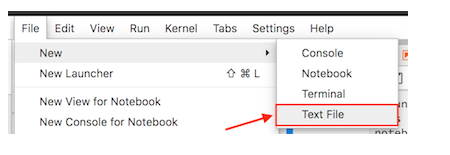
\includegraphics{./Figs/script1.png}
\end{frame}

\begin{frame}{Shkrimi i skripteve}
\protect\hypertarget{shkrimi-i-skripteve-4}{}
Kjo do të krijojë një fletë të re në dritaren tuaj të JupyterLab që
duhet të duket diçka e ngjashme me më poshtë, një hapësirë bosh.

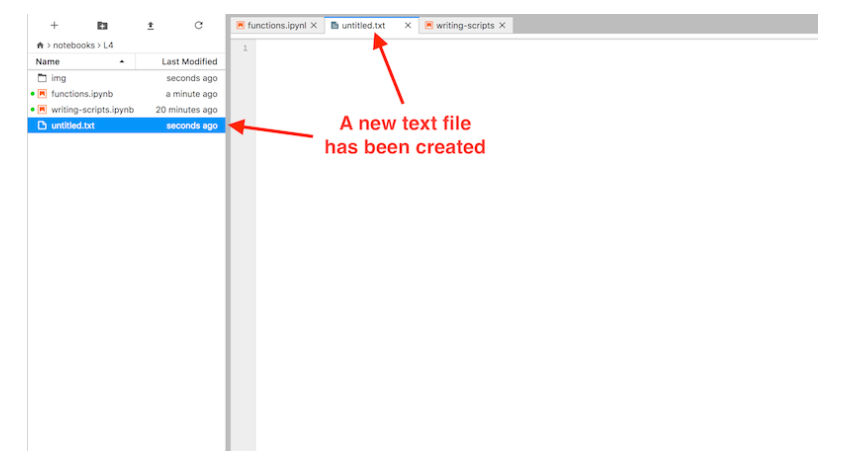
\includegraphics{./Figs/script2.png}
\end{frame}

\begin{frame}[fragile]{Shkrimi i skripteve}
\protect\hypertarget{shkrimi-i-skripteve-5}{}
Filloni duke kopjuar dhe ngjitur tekstin më poshtë në panelin e
redaktorit të fajlit tuaj të tekstit të ri.

\begin{Shaded}
\begin{Highlighting}[]

\KeywordTok{def}\NormalTok{ cels\_ne\_fahr(temp\_cels):}
    \ControlFlowTok{return} \DecValTok{9}\OperatorTok{/}\DecValTok{5} \OperatorTok{*}\NormalTok{ temp\_cels }\OperatorTok{+} \DecValTok{32}
\end{Highlighting}
\end{Shaded}
\end{frame}

\begin{frame}{Shkrimi i skripteve}
\protect\hypertarget{shkrimi-i-skripteve-6}{}
\begin{itemize}
\item
  Skriptet Python janë thjesht fajle teksti të rregullt me prapashtesën
  \textbf{.py} për t'i identifikuar ato si burime kod për Python-in.
\item
  Për tu siguruar që fajli ynë i ri tekst të njihet si një fajl burimi
  Python në JupyterLab, ne duhet ta riemërtojmë për të pasur një
  prapashtesë \textbf{.py}.
\item
  Mund ta riemërtoni fajlin duke djathtas-klikuar mbi skedën me titullin
  untitled.txt dhe duke e riemërtuar si temp\_converter.py.
\end{itemize}
\end{frame}

\begin{frame}{Shkrimi i skripteve}
\protect\hypertarget{shkrimi-i-skripteve-7}{}
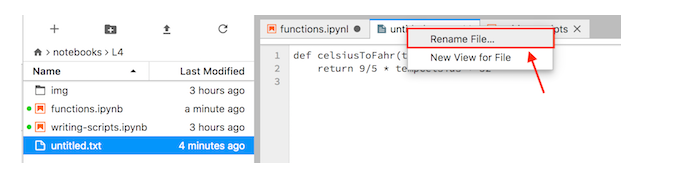
\includegraphics{./Figs/script3.png}
\end{frame}

\begin{frame}{Shkrimi i skripteve}
\protect\hypertarget{shkrimi-i-skripteve-8}{}
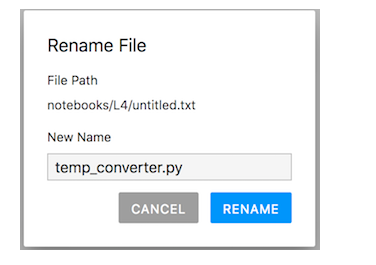
\includegraphics{./Figs/script4.png}
\end{frame}

\begin{frame}{Shkrimi i skripteve}
\protect\hypertarget{shkrimi-i-skripteve-9}{}
\begin{itemize}
\item
  Sigurohuni të ruani fajlin tuaj \textbf{temp\_converter.py} pasi të
  kryeni ndryshimet.
\item
  Nëse gjithçka shkon mirë, tani duhet të shihni sintaksën Python që
  është shënuar në ngjyra të ndryshme në panelin e redaktimit të
  JupyterLab.
\end{itemize}
\end{frame}

\begin{frame}{Ruajtja dhe ngarkimi i funksioneve}
\protect\hypertarget{ruajtja-dhe-ngarkimi-i-funksioneve}{}
\begin{itemize}
\item
  Natyrisht, pasi të keni ruajtur funksionet si ato më sipër në një fajl
  skripti, është e rëndësishme të dini si ti përdorim.
\item
  Siç u tha më herët, shpesh është e dobishme të krijohet një bibliotekë
  funksionesh të dedikuar për funksionet që përdorni shpesh.
\end{itemize}
\end{frame}

\begin{frame}{Ruajtja e funksioneve në një skript}
\protect\hypertarget{ruajtja-e-funksioneve-nuxeb-njuxeb-skript}{}
\begin{itemize}
\item
  Para se të vazhdojmë të diskutojmë se si të përdorim funksionet në
  skript, le të shtojmë disa funksione të tjera që kemi përdorur në
  leksionin tonë.
\item
  Thjesht kopjoni dhe ngjitni tekstin më poshtë në fajlin tuaj
  \textbf{temp\_converter.py}, duke lënë një vijë të zbrazët midis
  secilit funksion.
\end{itemize}
\end{frame}

\begin{frame}[fragile]{Ruajtja e funksioneve në një skript}
\protect\hypertarget{ruajtja-e-funksioneve-nuxeb-njuxeb-skript-1}{}
\begin{Shaded}
\begin{Highlighting}[]
\KeywordTok{def}\NormalTok{ cels\_ne\_fahr(temp\_cels):}
    \ControlFlowTok{return} \DecValTok{9}\OperatorTok{/}\DecValTok{5} \OperatorTok{*}\NormalTok{ temp\_cels }\OperatorTok{+} \DecValTok{32}

\KeywordTok{def}\NormalTok{ kelv\_ne\_cel(temp\_kelv):}
    \ControlFlowTok{return}\NormalTok{ temp\_kelv }\OperatorTok{{-}} \FloatTok{273.15}

\KeywordTok{def}\NormalTok{ kelv\_to\_fahr(temp\_kelv):}
\NormalTok{    temp\_cels }\OperatorTok{=}\NormalTok{ kelv\_to\_cel(temp\_kelv)}
\NormalTok{    temp\_fahr }\OperatorTok{=}\NormalTok{ cels\_ne\_fahr(temp\_cels)}
    \ControlFlowTok{return}\NormalTok{ temp\_fahr}
\end{Highlighting}
\end{Shaded}
\end{frame}

\begin{frame}{Ruajtja e funksioneve në një skript}
\protect\hypertarget{ruajtja-e-funksioneve-nuxeb-njuxeb-skript-2}{}
\begin{itemize}
\item
  Për të thirrur funksionet nga skripti, fillimisht është e rëndësishme
  të sigurohemi që jemi në direktorinë e duhur për punën tonë.
\item
  Kemi nevojë të ndryshojmë direktorinë e punës në Jupyter Lab që të
  jetë ai ku ndodhet fajli \textbf{temp\_converter.py}.
\end{itemize}
\end{frame}

\begin{frame}[fragile]{Ruajtja e funksioneve në një skript}
\protect\hypertarget{ruajtja-e-funksioneve-nuxeb-njuxeb-skript-3}{}
Mund të shikojmë cilat fajla janë të pranishme në direktorinë ku jemi
duke përdorur një komandë magjike të IPython quajtur \textbf{\%ls}.

\begin{Shaded}
\begin{Highlighting}[]
\OperatorTok{\%}\NormalTok{ls}
\end{Highlighting}
\end{Shaded}
\end{frame}

\begin{frame}[fragile]{Importimi i Funksioneve nga një Skedar tjetër}
\protect\hypertarget{importimi-i-funksioneve-nga-njuxeb-skedar-tjetuxebr}{}
\begin{itemize}
\item
  Për të importuar një funksion nga një skedar tjetër, mund të përdorim
  një deklaratë importimi.
\item
  Le të importojmë funksionin \texttt{cels\_ne\_fahr()} nga skedari
  \texttt{temp\_converter.py} duke përdorur kodin më poshtë:
\end{itemize}

\begin{Shaded}
\begin{Highlighting}[]
\ImportTok{from}\NormalTok{ temp\_converter }\ImportTok{import}\NormalTok{ cels\_ne\_fahr}
\end{Highlighting}
\end{Shaded}
\end{frame}

\begin{frame}[fragile]{Përdorimi i Funksioneve të Importuara}
\protect\hypertarget{puxebrdorimi-i-funksioneve-tuxeb-importuara}{}
\begin{itemize}
\item
  Tani mund të përdorim funksionin e importuar për të llogaritur
  temperaturën në Fahrenheit ku uji ngrin.
\item
  Le të shohim shembullin më poshtë që përdor funksionin
  \texttt{cels\_ne\_fahr()}:
\end{itemize}
\end{frame}

\begin{frame}[fragile]{Përdorimi i Funksioneve të Importuara}
\protect\hypertarget{puxebrdorimi-i-funksioneve-tuxeb-importuara-1}{}
\begin{Shaded}
\begin{Highlighting}[]
\BuiltInTok{print}\NormalTok{(}\StringTok{"The freezing point of water in Fahrenheit is:"}\NormalTok{, cels\_ne\_fahr(}\DecValTok{0}\NormalTok{))}
\end{Highlighting}
\end{Shaded}
\end{frame}

\begin{frame}{Importimi i Shumë Funksioneve}
\protect\hypertarget{importimi-i-shumuxeb-funksioneve}{}
\begin{itemize}
\item
  Gjithashtu, është e mundur të importoni disa funksione njëherësh duke
  i ndarë me presje.
\item
  Nëse duam të importojmë të gjitha funksionet nga një skedar, mund të
  përdorim një tjetër deklaratë importimi.
\item
  Le të importojmë të gjitha funksionet nga \textbf{temp\_converter.py}
  me pseudonimin \textbf{tc}:
\end{itemize}
\end{frame}

\begin{frame}[fragile]{Importimi i Shumë Funksioneve}
\protect\hypertarget{importimi-i-shumuxeb-funksioneve-1}{}
\begin{Shaded}
\begin{Highlighting}[]
\ImportTok{import}\NormalTok{ temp\_converter }\ImportTok{as}\NormalTok{ tc}
\end{Highlighting}
\end{Shaded}

Tani mund të përdorim funksionet nga tc, siç është bërë më poshtë:
\end{frame}

\begin{frame}[fragile]{Importimi i Shumë Funksioneve}
\protect\hypertarget{importimi-i-shumuxeb-funksioneve-2}{}
\begin{Shaded}
\begin{Highlighting}[]
\BuiltInTok{print}\NormalTok{(}\StringTok{"Pika e ngrirjes së ujit në Fahrenheit është:"}\NormalTok{, tc.cels\_ne\_fahr(}\DecValTok{0}\NormalTok{))}
\end{Highlighting}
\end{Shaded}
\end{frame}

\begin{frame}{Krijimi i një Funksioni të Ri}
\protect\hypertarget{krijimi-i-njuxeb-funksioni-tuxeb-ri}{}
\begin{itemize}
\item
  Tani do të krijojmë një funksion të ri që pranon temperatura në Kelvin
  dhe i konverton në Celsius ose Fahrenheit.
\item
  Funksioni do të quhet \textbf{temp\_calc} dhe do të ketë dy parametra:
  \textbf{temp\_k} për temperaturën në Kelvin dhe \textbf{convert\_to}
  për të zgjedhur llojin e konvertimit.
\end{itemize}
\end{frame}

\begin{frame}[fragile]{Krijimi i një Funksioni të Ri}
\protect\hypertarget{krijimi-i-njuxeb-funksioni-tuxeb-ri-1}{}
\begin{Shaded}
\begin{Highlighting}[]
\KeywordTok{def}\NormalTok{ temp\_calc(temp\_k, convert\_to):}
    \CommentTok{\# Check if user wants the temperature in Celsius}
    \ControlFlowTok{if}\NormalTok{ convert\_to }\OperatorTok{==} \StringTok{"C"}\NormalTok{:}
        \CommentTok{\# Convert the value to Celsius using the dedicated function for the task that we imported from another script}
\NormalTok{        converted\_temp }\OperatorTok{=}\NormalTok{ kelv\_ne\_cel(temp\_kelv}\OperatorTok{=}\NormalTok{temp\_k)}
    \ControlFlowTok{elif}\NormalTok{ convert\_to }\OperatorTok{==} \StringTok{"F"}\NormalTok{:}
        \CommentTok{\# Convert the value to Fahrenheit using the dedicated function for the task that we imported from another script}
\NormalTok{        converted\_temp }\OperatorTok{=}\NormalTok{ kelv\_ne\_fahr(temp\_kelv}\OperatorTok{=}\NormalTok{temp\_k)}
    \CommentTok{\# Return the result}
    \ControlFlowTok{return}\NormalTok{ converted\_temp}
\end{Highlighting}
\end{Shaded}
\end{frame}

\begin{frame}[fragile]{Krijimi i një Funksioni të Ri}
\protect\hypertarget{krijimi-i-njuxeb-funksioni-tuxeb-ri-2}{}
Nëse duam të marrim temperaturën absolute zero në Celsius, mund të
përdorim funksionin e ri si në shembullin më poshtë:

\begin{Shaded}
\begin{Highlighting}[]
\BuiltInTok{print}\NormalTok{(}\StringTok{"Absolut zero në Celsius është:"}\NormalTok{, temp\_calc(}\DecValTok{0}\NormalTok{, }\StringTok{"C"}\NormalTok{))}
\end{Highlighting}
\end{Shaded}
\end{frame}

\begin{frame}[fragile]{Krijimi i një Funksioni të Ri}
\protect\hypertarget{krijimi-i-njuxeb-funksioni-tuxeb-ri-3}{}
Tani, për të marrë temperaturën absolute zero në Fahrenheit:

\begin{Shaded}
\begin{Highlighting}[]
\BuiltInTok{print}\NormalTok{(}\StringTok{"Absolut zero në Fahrenheit është:"}\NormalTok{, temp\_calc(}\DecValTok{0}\NormalTok{, }\StringTok{"F"}\NormalTok{))}
\end{Highlighting}
\end{Shaded}
\end{frame}

\hypertarget{modulet}{%
\section{Modulet}\label{modulet}}

\begin{frame}{Përdorimi i Moduleve në Python}
\protect\hypertarget{puxebrdorimi-i-moduleve-nuxeb-python}{}
\begin{itemize}
\item
  Në këtë pjesë, ne do të shohim disa informacione rreth ngarkimit dhe
  përdorimit të moduleve në Python.
\item
  Një modul në Python është një pjesë kodi që përmban funksione dhe
  deklarata për të kryer detyra specifike.
\item
  Python ka shumë module të gatshme që mund të përdoren për detyra të
  ndryshme, gjë që e bën Python shumë fleksibël.
\end{itemize}
\end{frame}

\begin{frame}[fragile]{Çfarë janë Modulet, Paketat dhe Libraritë?}
\protect\hypertarget{uxe7faruxeb-januxeb-modulet-paketat-dhe-librarituxeb}{}
\begin{itemize}
\item
  \textbf{Moduli} është një skedar Python që përmban funksione dhe
  deklarata (p.sh., \texttt{.py}).
\item
  \textbf{Paketa} është një mënyrë për të organizuar module në entitete
  më të mëdha.
\item
  \textbf{Biblioteka} është një term i përgjithshëm që i referohet
  grupeve të moduleve ose paketave që kryejnë detyra specifike.
\end{itemize}
\end{frame}

\begin{frame}[fragile]{Ngarkimi i Moduleve}
\protect\hypertarget{ngarkimi-i-moduleve}{}
\begin{itemize}
\item
  Modulet ngarkohen me deklaratën \texttt{import}.
\item
  Shembull: Ngarkimi i modulit \texttt{math} dhe përdorimi i funksionit
  \texttt{sqrt()}:
\end{itemize}

\begin{Shaded}
\begin{Highlighting}[]
  \ImportTok{import}\NormalTok{ math}
\NormalTok{  math.sqrt(}\DecValTok{81}\NormalTok{)}
\end{Highlighting}
\end{Shaded}
\end{frame}

\begin{frame}[fragile]{Funksionet Built-In}
\protect\hypertarget{funksionet-built-in}{}
\begin{itemize}
\item
  Disa funksione janë të ndërtuara dhe nuk kërkojnë importim.
\item
  Shembull: Funksioni \textbf{print()} për të shtypur tekst në konsolë:
\end{itemize}

\begin{Shaded}
\begin{Highlighting}[]
\BuiltInTok{print}\NormalTok{(}\StringTok{"Hello world!"}\NormalTok{)}
\end{Highlighting}
\end{Shaded}
\end{frame}

\begin{frame}[fragile]{Riemërtimi i Moduleve}
\protect\hypertarget{riemuxebrtimi-i-moduleve}{}
\begin{itemize}
\item
  Mund të riemërtoni modulet për t'i bërë më të lehta për t'u përdorur.
\item
  Shembull: Riemërtimi i \textbf{math} në \textbf{m} dhe përdorimi i
  funksionit \textbf{sqrt()}:
\end{itemize}

\begin{Shaded}
\begin{Highlighting}[]
\ImportTok{import}\NormalTok{ math }\ImportTok{as}\NormalTok{ m}
\NormalTok{m.sqrt(}\DecValTok{49}\NormalTok{)}
\end{Highlighting}
\end{Shaded}
\end{frame}

\begin{frame}[fragile]{Importimi i Një Funksioni të Vetëm}
\protect\hypertarget{importimi-i-njuxeb-funksioni-tuxeb-vetuxebm}{}
\begin{itemize}
\item
  Mund të importoni një funksion të vetëm nga një modul.
\item
  Shembull: Importimi i sqrt() nga math:
\end{itemize}

\begin{Shaded}
\begin{Highlighting}[]
\ImportTok{from}\NormalTok{ math }\ImportTok{import}\NormalTok{ sqrt}
\NormalTok{sqrt(}\DecValTok{121}\NormalTok{)}
\end{Highlighting}
\end{Shaded}
\end{frame}

\begin{frame}[fragile]{Importimi i Nënmoduleve}
\protect\hypertarget{importimi-i-nuxebnmoduleve}{}
\begin{itemize}
\item
  Disa module kanë nënmodule që mund të importohen veçmas.
\item
  Shembull: Importimi i pyplot nga matplotlib për të bërë grafika:
\end{itemize}

\begin{Shaded}
\begin{Highlighting}[]
\ImportTok{import}\NormalTok{ matplotlib.pyplot }\ImportTok{as}\NormalTok{ plt}
\NormalTok{plt.plot([}\DecValTok{1}\NormalTok{, }\DecValTok{2}\NormalTok{, }\DecValTok{3}\NormalTok{, }\DecValTok{4}\NormalTok{, }\DecValTok{5}\NormalTok{], [}\DecValTok{5}\NormalTok{, }\DecValTok{2}\NormalTok{, }\DecValTok{3}\NormalTok{, }\DecValTok{4}\NormalTok{, }\DecValTok{1}\NormalTok{])}
\end{Highlighting}
\end{Shaded}
\end{frame}

\begin{frame}[fragile]{Kontrollimi i Funksioneve dhe Moduleve të
Disponueshme}
\protect\hypertarget{kontrollimi-i-funksioneve-dhe-moduleve-tuxeb-disponueshme}{}
\begin{itemize}
\item
  Për të parë funksionet në një modul, mund të përdorni dir().
\item
  Shembull: Kontrollimi i funksioneve në modulit math:
\end{itemize}

\begin{Shaded}
\begin{Highlighting}[]
\BuiltInTok{dir}\NormalTok{(math)}
\end{Highlighting}
\end{Shaded}
\end{frame}

\begin{frame}{Çfarë të Shmangni?}
\protect\hypertarget{uxe7faruxeb-tuxeb-shmangni}{}
\begin{itemize}
\item
  Mos përdorni from X import *, pasi kjo mund të shkaktojë konflikte
  emërimesh.
\item
  Përdorni emra të qartë kur riemërtoni modulet.
\item
  Importoni modulet në fillim të skedarit, sipas praktikave të mira të
  kodimit.
\end{itemize}
\end{frame}

\hypertarget{praktikuxeb}{%
\section{Praktikë}\label{praktikuxeb}}

\begin{frame}{Ushtrimi 1 - Fillimi me Python}
\protect\hypertarget{ushtrimi-1---fillimi-me-python}{}
Qëllimi i këtij ushtrimi është të shtypësh tekst në ekran bazuar në
vlerat e variablave që ke përcaktuar.
\end{frame}

\begin{frame}[fragile]{Pjesët që duhen bërë:}
\protect\hypertarget{pjesuxebt-quxeb-duhen-buxebruxeb}{}
\begin{itemize}
\item
  Krijo tre variabla: një numër të plotë për vlerësimin e kafes, një
  numër të plotë për vlerësimin e gjumit, dhe një varg karakteresh për
  emrin tënd.
\item
  Llogarit mesataren e dy vlerësimeve dhe ruaje rezultatin në një
  variabël për lumturinë.
\item
  Gjej tipin e të dhënave për secilin variabël. A ka ndonjë befasi?
\item
  Riprodho tekstin e shembullit duke përdorur funksionin
  \texttt{print()} dhe variablat që ke përcaktuar.
\end{itemize}
\end{frame}

\begin{frame}[fragile]{Zgjidhje:}
\protect\hypertarget{zgjidhje}{}
\begin{Shaded}
\begin{Highlighting}[]
\NormalTok{emri }\OperatorTok{=} \StringTok{"Endri"}
\NormalTok{vleresimi\_kafe }\OperatorTok{=} \DecValTok{9}
\NormalTok{vleresimi\_gjumit }\OperatorTok{=} \DecValTok{8}
\NormalTok{lumturia }\OperatorTok{=}\NormalTok{ (vleresimi\_kafe }\OperatorTok{+}\NormalTok{ vleresimi\_gjumit) }\OperatorTok{/} \DecValTok{2}

\BuiltInTok{print}\NormalTok{(}\SpecialStringTok{f"Emri im është }\SpecialCharTok{\{}\NormalTok{emri}\SpecialCharTok{\}}\SpecialStringTok{ dhe i jap pirjes të kafes një vlerësim prej }\SpecialCharTok{\{}\NormalTok{vleresimi\_kafe}\SpecialCharTok{\}}\SpecialStringTok{ nga 10!"}\NormalTok{)}
\BuiltInTok{print}\NormalTok{(}\SpecialStringTok{f"Vlerësimi im për kënaqësinë e gjumit është }\SpecialCharTok{\{}\NormalTok{vleresimi\_gjumit}\SpecialCharTok{\}}\SpecialStringTok{ / 10!"}\NormalTok{)}
\BuiltInTok{print}\NormalTok{(}\SpecialStringTok{f"Duke u bazuar në faktorët e mësipërm, vlerësimi im për lumturinë është }\SpecialCharTok{\{}\NormalTok{lumturia}\SpecialCharTok{\}}\SpecialStringTok{ nga 10 ose }\SpecialCharTok{\{}\NormalTok{lumturia }\OperatorTok{*} \DecValTok{10}\SpecialCharTok{\}}\SpecialStringTok{ \%!"}\NormalTok{)}
\end{Highlighting}
\end{Shaded}
\end{frame}

\begin{frame}{Ushtrimi 2 - Krijimi dhe Ndryshimi i Listave}
\protect\hypertarget{ushtrimi-2---krijimi-dhe-ndryshimi-i-listave}{}
Në këtë ushtrim, do të përdorësh të dhënat nga tabela për të krijuar
lista për emrat e stacioneve dhe vitet e para të funksionimit.

\begin{longtable}[]{@{}lll@{}}
\toprule\noalign{}
Emri i Stacionit FM & Viti i Parë i Trasmetimit & Grupi \\
\midrule\noalign{}
\endhead
TopRadio & 2003 & 1 \\
Energy & 2001 & 1 \\
Shqip FM & 2016 & 1 \\
Klan & 2005 & 1 \\
City FM & 2010 & 1 \\
Tirana & 2009 & 2 \\
BBF & 2012 & 2 \\
Magic FM & 2013 & 2 \\
\bottomrule\noalign{}
\end{longtable}
\end{frame}

\begin{frame}{Pjesët që duhen bërë:}
\protect\hypertarget{pjesuxebt-quxeb-duhen-buxebruxeb-1}{}
\begin{itemize}
\item
  Krijo dy lista: një për emrat e stacioneve dhe një për vitet e para të
  funksionimit për stacionet në Grupin 1.
\item
  Modifiko listat që sapo krijove për të shtuar vlerat nga Grupi 2.
\item
  Radhit listat: radhit listën e emrave në mënyrë alfabetike dhe listën
  e viteve që të fillojë me vitin më të fundit.
\end{itemize}
\end{frame}

\begin{frame}[fragile]{Shembull:}
\protect\hypertarget{shembull-2}{}
\begin{Shaded}
\begin{Highlighting}[]
\NormalTok{emrat\_grupi\_1 }\OperatorTok{=}\NormalTok{ [}\StringTok{"lighthouse"}\NormalTok{, }\StringTok{"Harmaja"}\NormalTok{, }\StringTok{"Suomenlinna aaltopoiju"}\NormalTok{, }\StringTok{"Kumpula"}\NormalTok{, }\StringTok{"Kaisaniemi"}\NormalTok{]}
\NormalTok{vitet\_grupi\_1 }\OperatorTok{=}\NormalTok{ [}\DecValTok{2003}\NormalTok{, }\DecValTok{1989}\NormalTok{, }\DecValTok{2016}\NormalTok{, }\DecValTok{2005}\NormalTok{, }\DecValTok{1844}\NormalTok{]}

\NormalTok{emrat\_grupi\_2 }\OperatorTok{=}\NormalTok{ [}\StringTok{"Malmi airfield"}\NormalTok{, }\StringTok{"Vuosaari harbour"}\NormalTok{, }\StringTok{"Kaivopuisto"}\NormalTok{]}
\NormalTok{vitet\_grupi\_2 }\OperatorTok{=}\NormalTok{ [}\DecValTok{1937}\NormalTok{, }\DecValTok{2012}\NormalTok{, }\DecValTok{1904}\NormalTok{]}
\end{Highlighting}
\end{Shaded}
\end{frame}

\begin{frame}[fragile]{Shembull:}
\protect\hypertarget{shembull-3}{}
\begin{Shaded}
\begin{Highlighting}[]
\CommentTok{\# Shtimi i Grupeve 2}
\NormalTok{emrat\_grupi\_1.extend(emrat\_grupi\_2)}
\NormalTok{vitet\_grupi\_1.extend(vitet\_grupi\_2)}

\CommentTok{\# Radhitja e listave}
\NormalTok{emrat\_grupi\_1.sort()  }\CommentTok{\# Radhitje alfabetike}
\NormalTok{vitet\_grupi\_1.sort(reverse}\OperatorTok{=}\VariableTok{True}\NormalTok{)  }\CommentTok{\# Viti më i fundit në fillim}
\end{Highlighting}
\end{Shaded}
\end{frame}

\begin{frame}{Ushtrimi 3 - Listat dhe Vlerat e Indeksit}
\protect\hypertarget{ushtrimi-3---listat-dhe-vlerat-e-indeksit}{}
Në këtë ushtrim, do të përdorësh të dhënat nga Tabela 2.6 për të krijuar
lista me muajt dhe temperaturat mesatare.
\end{frame}

\begin{frame}{Pjesët që duhen bërë:}
\protect\hypertarget{pjesuxebt-quxeb-duhen-buxebruxeb-2}{}
\begin{itemize}
\item
  Krijo dy lista me muajt dhe temperaturat mesatare.
\item
  Përdor një deklaratë print() për të prodhuar rezultatet bazuar në
  indeksin e listave.
\end{itemize}
\end{frame}

\begin{frame}[fragile]{Shembull:}
\protect\hypertarget{shembull-4}{}
\begin{Shaded}
\begin{Highlighting}[]
\NormalTok{muaj }\OperatorTok{=}\NormalTok{ [}\StringTok{"Janar"}\NormalTok{, }\StringTok{"Shkurt"}\NormalTok{, }\StringTok{"Mars"}\NormalTok{, }\StringTok{"Prill"}\NormalTok{, }\StringTok{"Maj"}\NormalTok{, }\StringTok{"Qershor"}\NormalTok{, }\StringTok{"Korrik"}\NormalTok{, }\StringTok{"Gusht"}\NormalTok{, }\StringTok{"Shtator"}\NormalTok{, }\StringTok{"Tetor"}\NormalTok{, }\StringTok{"Nëntor"}\NormalTok{, }\StringTok{"Dhjetor"}\NormalTok{]}
\NormalTok{temperatura }\OperatorTok{=}\NormalTok{ [}\OperatorTok{{-}}\FloatTok{3.5}\NormalTok{, }\OperatorTok{{-}}\FloatTok{4.5}\NormalTok{, }\OperatorTok{{-}}\FloatTok{1.0}\NormalTok{, }\FloatTok{4.0}\NormalTok{, }\FloatTok{10.0}\NormalTok{, }\FloatTok{15.0}\NormalTok{, }\FloatTok{18.0}\NormalTok{, }\FloatTok{16.0}\NormalTok{, }\FloatTok{11.5}\NormalTok{, }\FloatTok{6.0}\NormalTok{, }\FloatTok{2.0}\NormalTok{, }\OperatorTok{{-}}\FloatTok{1.5}\NormalTok{]}

\BuiltInTok{print}\NormalTok{(}\SpecialStringTok{f"Temperatura mesatare në Tiranë në }\SpecialCharTok{\{}\NormalTok{muajt[}\DecValTok{2}\NormalTok{]}\SpecialCharTok{\}}\SpecialStringTok{ është }\SpecialCharTok{\{}\NormalTok{temperaturat[}\DecValTok{2}\NormalTok{]}\SpecialCharTok{\}}\SpecialStringTok{"}\NormalTok{)}
\end{Highlighting}
\end{Shaded}
\end{frame}

\begin{frame}{Ushtrimi 4 - Përpunimi me një Cikël for}
\protect\hypertarget{ushtrimi-4---puxebrpunimi-me-njuxeb-cikuxebl-for}{}
\begin{itemize}
\tightlist
\item
  Në këtë ushtrim, synohet të krijosh një listë me emra skedarësh që
  mund të përdoren për të përpunuar të dhënat me një cikël for.
\end{itemize}
\end{frame}

\begin{frame}{Pjesët që duhen bërë:}
\protect\hypertarget{pjesuxebt-quxeb-duhen-buxebruxeb-3}{}
\begin{itemize}
\tightlist
\item
  Përdor një cikël for për të krijuar një listë me emra skedarësh.
\end{itemize}
\end{frame}

\begin{frame}[fragile]{Shembull:}
\protect\hypertarget{shembull-5}{}
\begin{Shaded}
\begin{Highlighting}[]
\NormalTok{emrat\_skedareve }\OperatorTok{=}\NormalTok{ [}\SpecialStringTok{f"Station\_}\SpecialCharTok{\{}\NormalTok{i}\SpecialCharTok{\}}\SpecialStringTok{.txt"}\NormalTok{ për i në varg(}\DecValTok{21}\NormalTok{)]}

\BuiltInTok{print}\NormalTok{(emrat\_skedareve)}
\end{Highlighting}
\end{Shaded}
\end{frame}

\begin{frame}{Ushtrimi 5 - Klasifikimi i Temperaturave}
\protect\hypertarget{ushtrimi-5---klasifikimi-i-temperaturave}{}
\begin{itemize}
\tightlist
\item
  Në këtë ushtrim, do të përdorësh një cikël for dhe deklarata if, elif,
  else për të klasifikuar temperaturat në lista të ndryshme.
\end{itemize}
\end{frame}

\begin{frame}{Pjesët që duhen bërë:}
\protect\hypertarget{pjesuxebt-quxeb-duhen-buxebruxeb-4}{}
\begin{itemize}
\item
  Krijo lista bosh për secilën kategori: ``cold'', ``slippery'',
  ``comfortable'', ``warm''.
\item
  Klasifiko temperaturat në lista për secilën kategori.
\end{itemize}
\end{frame}

\begin{frame}[fragile]{Shembull:}
\protect\hypertarget{shembull-6}{}
\begin{Shaded}
\begin{Highlighting}[]
\NormalTok{temperaturat }\OperatorTok{=}\NormalTok{ [}\OperatorTok{{-}}\FloatTok{5.4}\NormalTok{, }\FloatTok{1.0}\NormalTok{, }\OperatorTok{{-}}\FloatTok{1.3}\NormalTok{, }\OperatorTok{{-}}\FloatTok{4.8}\NormalTok{, }\FloatTok{3.9}\NormalTok{, }\FloatTok{0.1}\NormalTok{, }\OperatorTok{{-}}\FloatTok{4.4}\NormalTok{, }\FloatTok{4.0}\NormalTok{, }\OperatorTok{{-}}\FloatTok{2.2}\NormalTok{, }\OperatorTok{{-}}\FloatTok{3.9}\NormalTok{, }\FloatTok{4.4}\NormalTok{]}

\NormalTok{ftohte }\OperatorTok{=}\NormalTok{ []}
\NormalTok{rreshqitje }\OperatorTok{=}\NormalTok{ []}
\NormalTok{rehat }\OperatorTok{=}\NormalTok{ []}
\NormalTok{ngrohte }\OperatorTok{=}\NormalTok{ []}

\ControlFlowTok{for}\NormalTok{ temp }\KeywordTok{in}\NormalTok{ temperaturat:}
    \ControlFlowTok{if}\NormalTok{ temp }\OperatorTok{\textless{}} \OperatorTok{{-}}\DecValTok{2}\NormalTok{:}
\NormalTok{        ftohte.append(temp)}
    \ControlFlowTok{elif} \OperatorTok{{-}}\DecValTok{2} \OperatorTok{\textless{}=}\NormalTok{ temp }\OperatorTok{\textless{}} \DecValTok{2}\NormalTok{:}
\NormalTok{        rreshqitje .append(temp)}
    \ControlFlowTok{elif} \DecValTok{2} \OperatorTok{\textless{}=}\NormalTok{ temp }\OperatorTok{\textless{}} \DecValTok{15}\NormalTok{:}
\NormalTok{        rehat.append(temp)}
    \ControlFlowTok{else}\NormalTok{:}
\NormalTok{        ngrohte.append(temp)}

\BuiltInTok{print}\NormalTok{(}\StringTok{"ftohte:"}\NormalTok{, ftohte)}
\BuiltInTok{print}\NormalTok{(}\StringTok{"rreshqitje:"}\NormalTok{, rreshqitje )}
\BuiltInTok{print}\NormalTok{(}\StringTok{"rehat:"}\NormalTok{, rehat)}
\BuiltInTok{print}\NormalTok{(}\StringTok{"ngrohte:"}\NormalTok{, ngrohte)}
\end{Highlighting}
\end{Shaded}
\end{frame}

\begin{frame}{Pyetje për t'u përgjigjur:}
\protect\hypertarget{pyetje-puxebr-tu-puxebrgjigjur}{}
\begin{itemize}
\item
  Sa herë ishte ftohtë në Tirane në Prill 2013?
\item
  Sa herë ishte rehat?
\item
  A ishte ndonjëherë ngrohtë?
\end{itemize}
\end{frame}

\begin{frame}{Një Funksion për Konvertimin e Temperaturave}
\protect\hypertarget{njuxeb-funksion-puxebr-konvertimin-e-temperaturave}{}
\begin{itemize}
\tightlist
\item
  Në këtë ushtrim, duhet të krijosh një funksion që konverton
  temperaturat nga Fahrenheit në Celsius.
\end{itemize}
\end{frame}

\begin{frame}{Pjesët që duhen bërë:}
\protect\hypertarget{pjesuxebt-quxeb-duhen-buxebruxeb-5}{}
\begin{itemize}
\item
  Krijo një funksion që konverton nga Fahrenheit në Celsius.
\item
  Përdor funksionin për të konvertuar temperaturat e mëposhtme në
  Celsius.
\end{itemize}
\end{frame}

\begin{frame}[fragile]{Shembull:}
\protect\hypertarget{shembull-7}{}
\begin{Shaded}
\begin{Highlighting}[]
\KeywordTok{def}\NormalTok{ fahrenheit\_ne\_celsius(temp\_fahr):}
    \CommentTok{"""}
\CommentTok{    Ky funksion konverton nga Fahrenheit në Celsius.}
\CommentTok{    """}
    \ControlFlowTok{return}\NormalTok{ (temp\_fahr }\OperatorTok{{-}} \DecValTok{32}\NormalTok{) }\OperatorTok{*}\NormalTok{ (}\DecValTok{5}\OperatorTok{/}\DecValTok{9}\NormalTok{)}

\NormalTok{temperatura\_1 }\OperatorTok{=}\NormalTok{ fahrenheit\_ne\_celsius(}\DecValTok{32}\NormalTok{)}
\NormalTok{temperatura\_2 }\OperatorTok{=}\NormalTok{ fahrenheit\_ne\_celsius(}\DecValTok{68}\NormalTok{)}
\NormalTok{temperatura\_3 }\OperatorTok{=}\NormalTok{ fahrenheit\_ne\_celsius(}\DecValTok{91}\NormalTok{)}
\NormalTok{temperatura\_4 }\OperatorTok{=}\NormalTok{ fahrenheit\_ne\_celsius(}\OperatorTok{{-}}\DecValTok{17}\NormalTok{)}

\BuiltInTok{print}\NormalTok{(}\StringTok{"Temperatura 1:"}\NormalTok{, temperatura\_1)}
\BuiltInTok{print}\NormalTok{(}\StringTok{"Temperatura 2:"}\NormalTok{, temperatura\_2)}
\BuiltInTok{print}\NormalTok{(}\StringTok{"Temperatura 3:"}\NormalTok{, temperatura\_3)}
\BuiltInTok{print}\NormalTok{(}\StringTok{"Temperatura 4:"}\NormalTok{, temperatura\_4)}
\end{Highlighting}
\end{Shaded}
\end{frame}

\begin{frame}{Ushtrimi 6 - Një Funksion për Klasifikimin e
Temperaturave}
\protect\hypertarget{ushtrimi-6---njuxeb-funksion-puxebr-klasifikimin-e-temperaturave}{}
\begin{itemize}
\tightlist
\item
  Ky ushtrim përdor të njëjtën logjikë si Ushtrimi 2.5, por tani duke
  përdorur një funksion për të klasifikuar temperaturat.
\end{itemize}
\end{frame}

\begin{frame}{Pjesët që duhen bërë:}
\protect\hypertarget{pjesuxebt-quxeb-duhen-buxebruxeb-6}{}
\begin{itemize}
\tightlist
\item
  Krijo një funksion që klasifikon temperaturat sipas Tabelës
\end{itemize}

\begin{longtable}[]{@{}
  >{\raggedright\arraybackslash}p{(\columnwidth - 4\tabcolsep) * \real{0.2167}}
  >{\raggedright\arraybackslash}p{(\columnwidth - 4\tabcolsep) * \real{0.5500}}
  >{\raggedright\arraybackslash}p{(\columnwidth - 4\tabcolsep) * \real{0.2333}}@{}}
\toprule\noalign{}
\begin{minipage}[b]{\linewidth}\raggedright
Kategoria
\end{minipage} & \begin{minipage}[b]{\linewidth}\raggedright
Gama e Temperaturës
\end{minipage} & \begin{minipage}[b]{\linewidth}\raggedright
Emri i Listës
\end{minipage} \\
\midrule\noalign{}
\endhead
Ftohtë & Më pak se -2 gradë C & cold \\
Rrëshqitëse & Më shumë ose e barabartë me -2 gradë C dhe më pak se +2
gradë C & slippery \\
Komode & Më shumë ose e barabartë me +2 gradë C dhe më pak se +15 gradë
C & comfortable \\
Ngrohtë & Më shumë ose e barabartë me +15 gradë C & warm \\
\bottomrule\noalign{}
\end{longtable}

Funksioni duhet të kthejë vlera të ndryshme për kategoritë e ndryshme.
\end{frame}

\begin{frame}[fragile]{Shembull:}
\protect\hypertarget{shembull-8}{}
\begin{Shaded}
\begin{Highlighting}[]

\NormalTok{def klasifikues\_temperaturash(temp):}
\NormalTok{    """}
\NormalTok{    Klasifikon temperaturat sipas kategorive të përcaktuara.}
\NormalTok{    Kthen një vlerë të ndryshme për çdo kategori.}
\NormalTok{    """}
\NormalTok{    if temp \textless{} {-}2:}
\NormalTok{        return 0  \# Ftohtë}
\NormalTok{    elif {-}2 \textless{}= temp \textless{} 2:}
\NormalTok{        return 1  \# Rrëshqitëse}
\NormalTok{    elif 2 \textless{}= temp \textless{} 15:}
\NormalTok{        return 2  \# Komode}
\NormalTok{    else:}
\NormalTok{        return 3  \# Ngrohtë}
\end{Highlighting}
\end{Shaded}
\end{frame}

\end{document}
